\section{Dislocation avalanche statistics and machine learning}
The result from MD and atomistic simulation like stress-strain and displacement-time graphs are used to generate the statistics of dislocation avalanches like size and velocity.

Dislocation avalanche size distribution can calculated from the stress-strain information. The magnitude of the dislocation slip is obtained by using Complementary Cumulative Distribution
Function (CCDF) C(S,$\sigma$) equ.(\ref{CCDF})$^{\cite{Hu2018}}$ which on using scaling factor would give the dislocation avalanche distribution based on slip size.$^{\cite{Hu2018}}$.where S is slip size and $\sigma$ is stress

\begin{equation}\label{CCDF}
C(S, \sigma) \sim \int_{S}^{\infty} D\left(S^{\prime}, \sigma\right) d S^{\prime} \sim S^{-(\kappa-1)} g\left(S\left(\sigma_{c}-\sigma\right)^{\frac{1}{\beta}}\right)
\end{equation}

The fact that the dislocation avalanches depends on the size distribution implies that two response regimes exist. After yield point, small avalanches can be regarded as precursor events or an incubation stage
leading up to the occasional major relaxation event. When the external force reaches a critical value all dislocation would glide continuously causing large dislocation avalanches having steady plastic flow. 

From displacement-time information, velocities of the dislocation avalanches are calculated. The probability of a certain displacement magnitude to occur follows a power-law distribution over at least two orders of magnitude.$^{\cite{MAA2013586}}$


\begin{wrapfigure}{R}{0.6\textwidth}
\centering
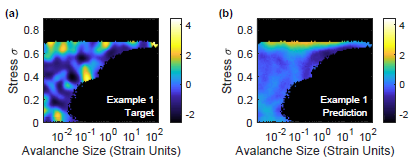
\includegraphics[width=0.65\textwidth]{section_4_1.png}
\caption{\label{fig:Simulation graph}stress-strain graph.$^{\cite{Fan2020}}$}
\end{wrapfigure}

Many supervised Machine Learning algorithms like neural network are capable of learning non-linear mapping of features to a desired output. Therefore, this method is used for predicting deformation.Due to dislocation avalanches there are irregularities in stress-strain relation as a result of strain bursts. These strain bursts follow power-law distribution until the system reaches criticality. The predictive model to simulate stress-strain curve can be achieved by using sample-specific information about the pinning landscape as well as the initial dislocation configuration as input. From these predicted stress-strain curves, the dislocation avalanche statistics can also be predicted.In figure (\ref{fig:Simulation graph}) using CNN we predicted strain bursts.

\textbf{Conculsion}: 





